\documentclass[10pt,a4paper,oneside,fleqn]{report}
\usepackage{geometry}
\geometry{a4paper,left=20mm,right=20mm,top=1cm,bottom=2cm}
\usepackage[utf8]{inputenc}
%\usepackage{ngerman}
\usepackage{amsmath}                % brauche ich um dir Formel zu umrahmen.
\usepackage{amsfonts}                % brauche ich für die Mengensymbole
\usepackage{graphicx}
\setlength{\parindent}{0px}
\setlength{\mathindent}{10mm}
\usepackage{bbold}                    %brauche ich für die doppel Zahlen Darstellung (Einheitsmatrix z.B)
\usepackage[linktocpage={false}]{hyperref}


\usepackage{color}
\usepackage{titlesec} %sudo apt-get install texlive-latex-extra

\definecolor{darkblue}{rgb}{0.1,0.1,0.55}
\definecolor{darkred}{rgb}{0.55,0.2,0.2}

\titleformat{\chapter}[display]{\color{darkred}\normalfont\huge\bfseries}{\chaptertitlename\
\thechapter}{20pt}{\Huge}

\titleformat{\section}{\color{darkblue}\normalfont\Large\bfseries}{\thesection}{1em}{}
\titleformat{\subsection}{\color{darkblue}\normalfont\Large\bfseries}{\thesection}{1em}{}

% Notiz Box
\usepackage{fancybox}
\newcommand{\notiz}[1]{\vspace{5mm}\ovalbox{\begin{minipage}{1\textwidth}#1\end{minipage}}\vspace{5mm}}

\usepackage{cancel}




\begin{document}
\tableofcontents
\setcounter{chapter}{5}
\chapter{Gitterdynamik und Phononen}

\section{Gitterschwingungen}

1D Kette mit einatomiger Basis. 

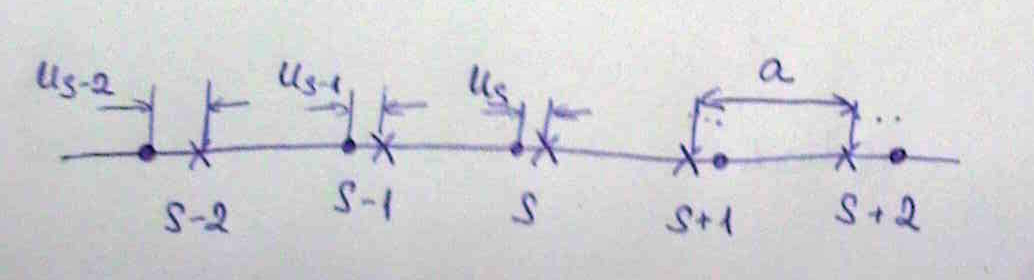
\includegraphics[width=0.75\textwidth]{kap06_01.png}

Bewegungsgleichungen:

\[ M\frac{d^2 u_s}{dt^2} = \sum^{\infty}_{n=-\infty}c_n(u_{s+n}-u_s)\]
mit \(c_n\) als Kraftkonstante

Lösung: \(u_{s+n}=v e^{-i\omega t + igna}\)

\[\omega^2 M = \sum^{\infty}_{n=-\infty}c_n(1-e^{iqna})\]

nach Symmetrie \(c_{-n}=c_n\)

\[\omega^2 = \frac{1}{M} \sum^{\infty}_{n=-\infty}c_n(2-e^{iqna}-e^{-iqna})=\frac{2}{M} \sum^{\infty}_{n=-\infty}c_n(2-cos(qna))\]
\(c_1 >> c_n\), für  \(n\geq 2\), nur nächst. Nachbarn \(\rightarrow \omega^2=\frac{2c_1}{M} (1-cos(qa)) =\frac{4c_1}{M} (sin^2(\frac{qa}{2}))\)

\[\omega = 2\sqrt{\frac{c_1}{M}}\left| sin\frac{qa}{2}\right|\]

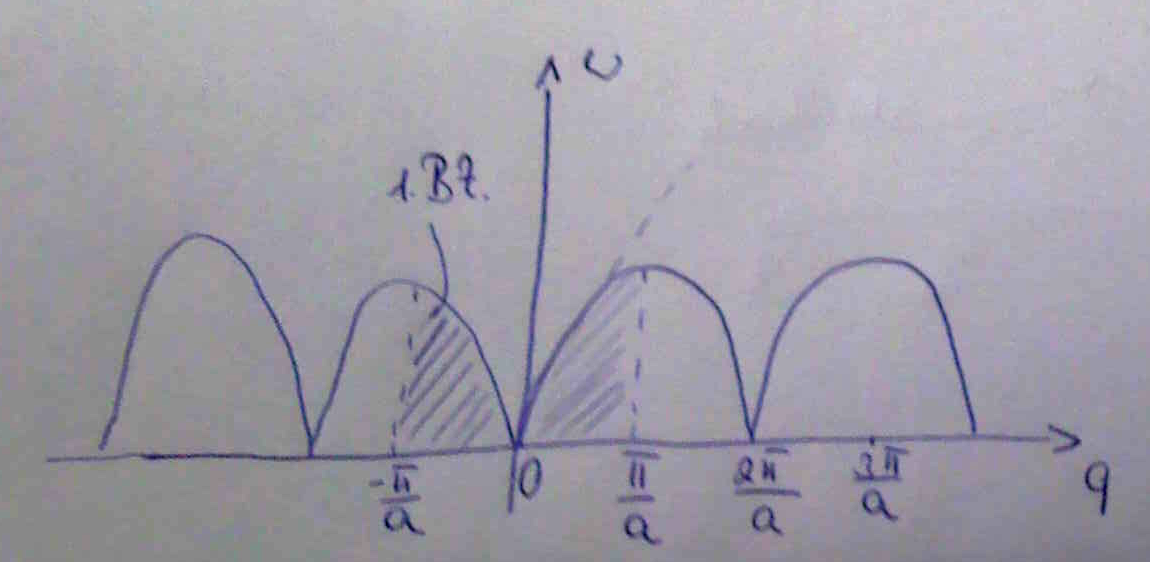
\includegraphics[width=0.75\textwidth]{kap06_02.png}

bei \(c_2\neq 0\); \(\omega^2 = \frac{4c_1}{M}\left[\ sin^2\frac{qa}{2} + \frac{c_2}{c_1}sin^2(qa) \right]\)

\(\frac{u_{s+1}}{u_s} = e^{iqa}\rightarrow\) Phasenunterschied

Wir betrachten den Bereich \(-\pi < qa < \pi\). Reduktion auf die 1. Brillouin-Zone; \(\underbrace{q'}_{\text{außerhalb 1 BZ}}=\underbrace{q}_{\text{1 BZ}}+\frac{2\pi N}{a}\) mit \(N\in \mathbb Z\)

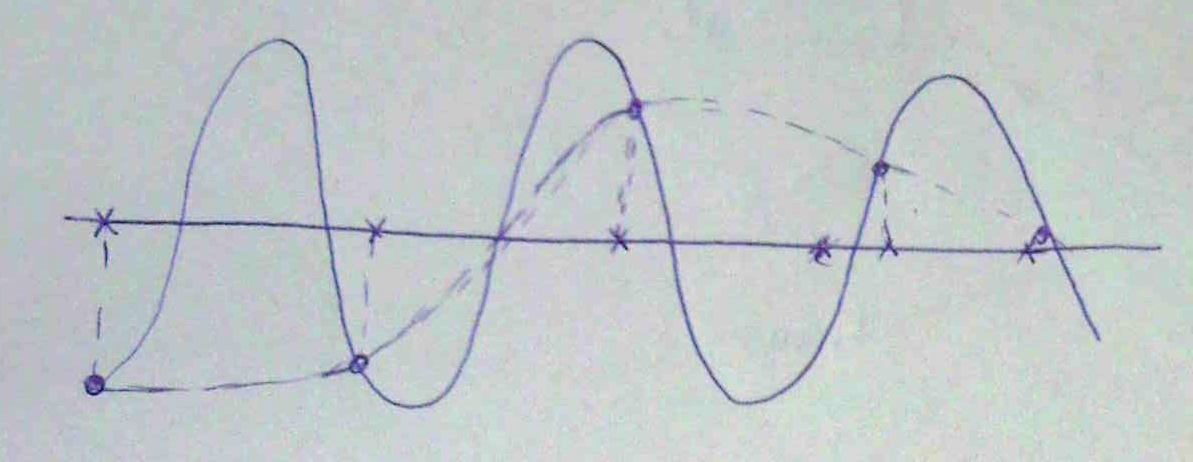
\includegraphics[width=0.75\textwidth]{kap06_03.png}

\(\frac{u_{s+1}}{u_s} = e^{iqa}\cdot e^{2\pi N}\)

- Gruppengeschwindigkeit: \(v_g = \frac{d\omega}{dq}\) (entspricht den Energietransport) (\(v_g=0\) eine Stehende Welle, Schwinung in Gegenphase, kein Energietransport)
- Phasengeschwindigkeit: \(v_{Ph} = \frac{\omega}{q}\)

Langwelliger Grenzfall: \(q\rightarrow 0\); \(\lambda \rightarrow \infty\)

\[\omega^2 = \frac{2}{M} \sum^{\infty}_{n=1}c_n(1-\underbrace{cos(qna)}_{\approx 1-\frac{x^2}{2}+...})\approx \frac{q^2a^2}{M}\sum^{\infty}_{n=1}n^2s_n\]
\[ c_{11} = \sum^{\infty}_{n=1} \frac{n^2}{a}c^2_n\]

kurzwelliger Grenzfall: \(|q|\approx \frac{\pi}{a}\); \(\lambda = 2a\)

 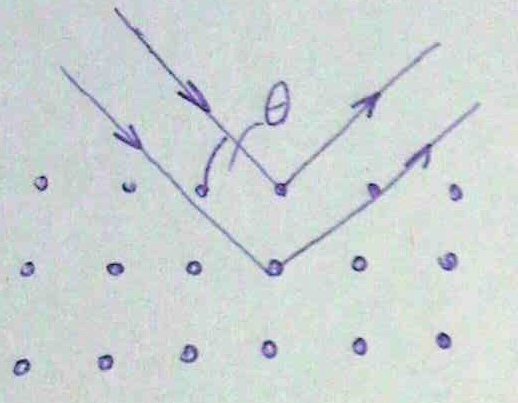
\includegraphics[width=0.75\textwidth]{kap06_04.png}

\(2dsin\theta=\lambda\); \(d=a\); \(\theta = \frac{\pi}{2}\)

\section{Gitter mit 2-Atomiger Basis}

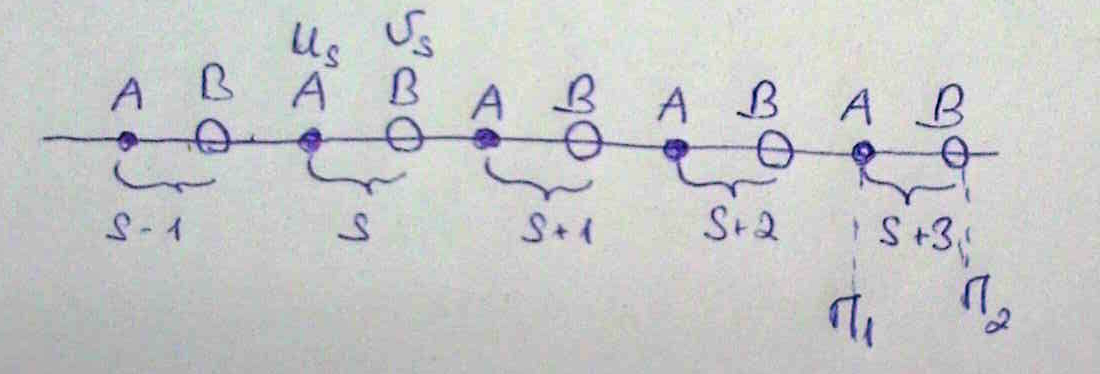
\includegraphics[width=0.75\textwidth]{kap06_05.png}

\[ M_1\frac{d^2 u_s}{dt^2} = c'(v_s-u_s)-c''(u_s-v_{s-1})\]
\[ M_2\frac{d^2 u_s}{dt^2} = c''(v_{s+1}-v_s)-c'(v_s-u_s)\]

Lösung \(u_s=ue^{-i\omega t + iqsa}\); \(v_s=ve^{-i\omega t + iqsa}\)



\(det|...|=0\); Eigenfrequenzen: \(\omega^2_{\pm} = \frac{\omega^2_0}{2}\left[1\pm \sqrt{1-\gamma^2 sin^2\frac{qa}{2}} \right]\)


\(\gamma = e \frac{\sqrt{c'c''}}{c'+c''}\cdot \frac{\sqrt{M'_1 M'_2}}{M_1+M_2}\); \(\omega_0 = (c'+c'')(\frac{1}{M_1}+\frac{1}{M_2})\)

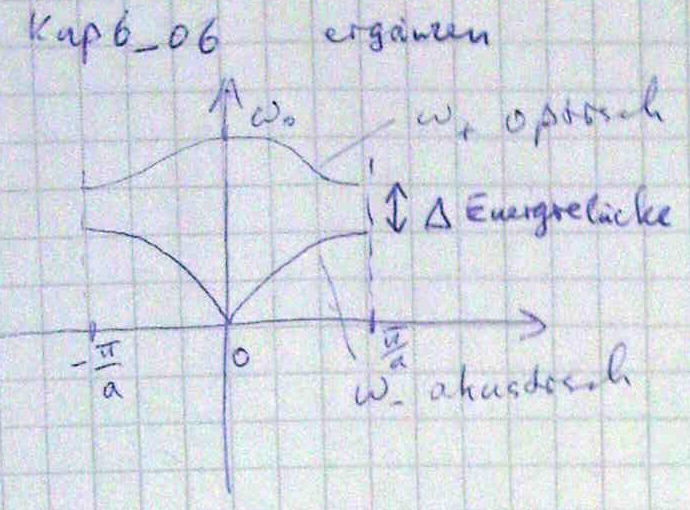
\includegraphics[width=0.75\textwidth]{kap06_06.png}


a) Für \(q\rightarrow 0\); \(\omega_0=\frac{2C}{\mu}\); \(c=c'=c''\); \(\mu^{-1}=\mu^{-1}_1+\mu^{-1}_2\)

\(\frac{u}{v}= -\frac{\mu_2}{\mu_1}\): Schwinung in Gegenphase; Ionenkristalle: oszillierendes elektrisches Dipolmoment

b) Für \(|q|\rightarrow \frac{\pi}{a}\); \(M_1<M_2\); \(\omega^2=\frac{2c}{M_1}\); \(\omega^2=\frac{2c}{M_2}\) \(\Rightarrow \frac{v}{u}=0\) bzw \(\frac{u}{v}=0\)

Frequenzlücke \(\rightarrow\) 'verbotene' Zone

\underline{3D Kristalle (mit P Atomen pro E.Z.)}

\begin{itemize}
\item Es gibt 3 akustische Zweige mit 1 longitudinale und 2 transversale
\item (3P-3) optische Zweige
\end{itemize}

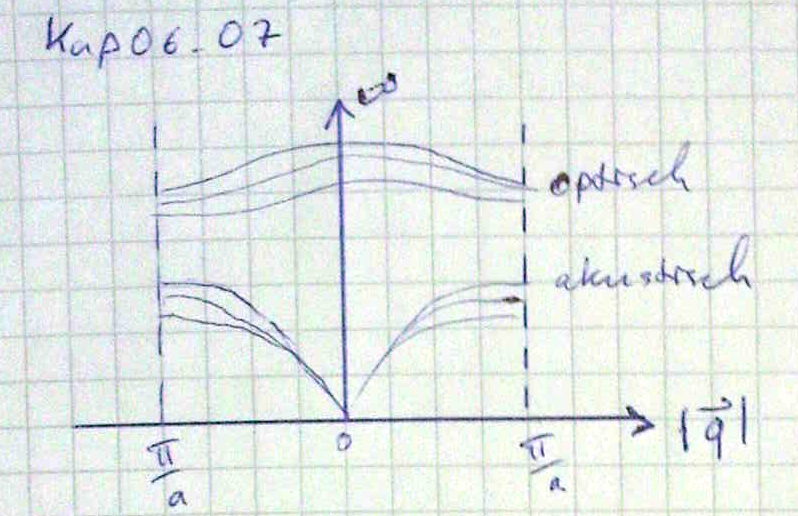
\includegraphics[width=0.75\textwidth]{kap06_07.png}

\section{Quanntisierung elastischer Wellen}

List (EM-Feld) \(\rightarrow\) Photonen \(\rightarrow\) Teilchen
Schall (elastisches Feld) \(\rightarrow\)  Phononen  \(\rightarrow\) Quasiteilchen

Quasiimpuls: \(\hbar \vec q\)
Energie: \(E_{\vec q}=\hbar \omega_{\vec q}\)

Quasiimpuls und seine Energie ist definiert nur in der 1.B.Z.

\[E_{\vec q}=\hbar(n_{\vec q}+\frac{1}{2})\omega_{\vec q}\]

Die Eigenwerte sind quantisiert

\(\frac{1}{2}\hbar \omega_{\vec q}\) ist die Nulpunktenergie des Schwingungszustandes

Energieverluste (inelast. Streuung)

Die Energieverluste könnten wir entweder klassisch (komplexe \(\omega,k\). Damit entspricht der Imaginäre-Teil den Verlusten. 

Oder die Energieverluste werden quantenmechanisch beschrieben (die Zahl der Teilchen ist reduziert). Inelastische Streuung durch Phononen representiert.

Impuls \(\underbrace{\vec k_0}_{\text{Photon}} + \underbrace{\vec B}_{\text{ein Vektor des reziproken Gitters}} = \vec k \pm \underbrace{\vec q}_{\text{Phonon mit Wellenvektor}\vec q}\); Energie \(\hbar \omega_0=\hbar\omega \pm \hbar \omega_q\) 

Ewald Konstruktion
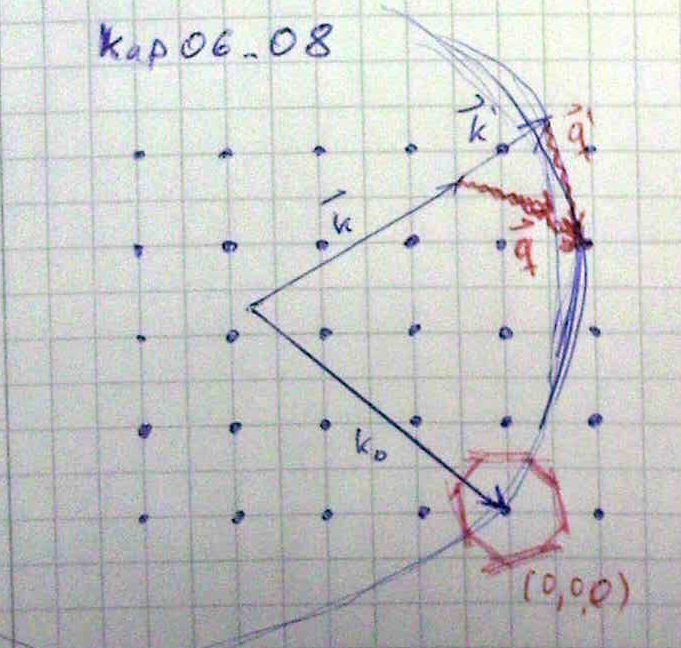
\includegraphics[width=0.75\textwidth]{kap06_08.png}

\(\oplus\) ein Phonon erzeugt
\(\ominus\) ein Phonon absorbiert

\underline{Widerholung} mögliche Streuteilchen (Messsonden)

\begin{itemize}
\item Röntgen-Photonen: \(E\approx 10keV\); ! Phononen: \(E_g\approx 10^{-2}eV\)
\item Elektronen: \(E\approx 100eV\); Nachteil die Eindringtiefe ist gering
\item Neutronen: \(E=\frac{p^2}{2m}=\frac{h^2}{2m\lambda^2} \approx 0,1eV\); können durch den ganzen körper praktisch ungehindert durchfliegen; können mit Phononen interaggieren (innelasische Streuung). 
\end{itemize}

Lichtstreuung: sichtbares List mit \(\lambda_\nu >> a\); \(|\vec k_0|<<|\vec B|\approx \frac{2\pi}{a}\), nur 1.B.Z.

Impulserhaltung: \(\vec k_0=\vec k \pm \vec q\)

Elastische Streuung: Rayleigh-Streuung \(\vec k=\vec k_0\); \(\vec q=0\)

Inelastische Streuprozesse:

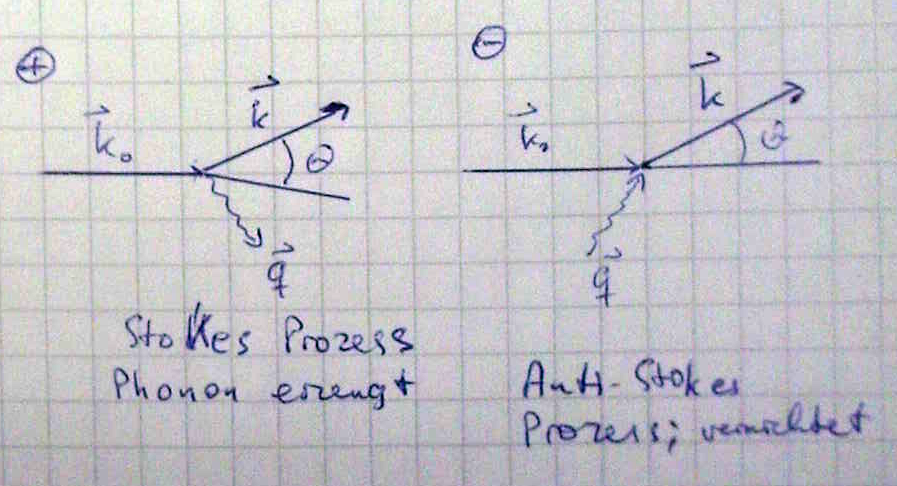
\includegraphics[width=0.75\textwidth]{kap06_09.png}

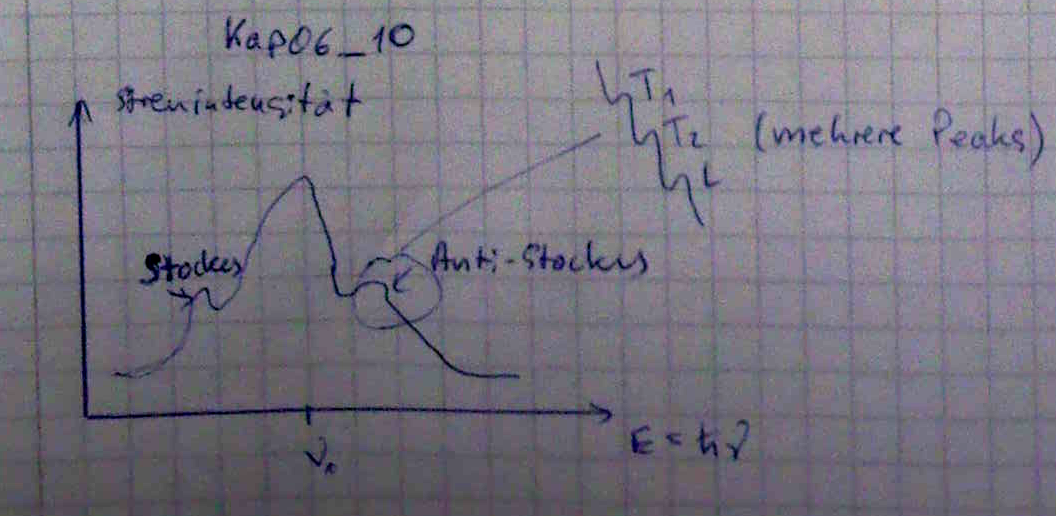
\includegraphics[width=0.75\textwidth]{kap06_10.png}

Streung an akustischen Phononen: Brilloiu-Streuung
Streung an optischen Phononen: Raman Streung

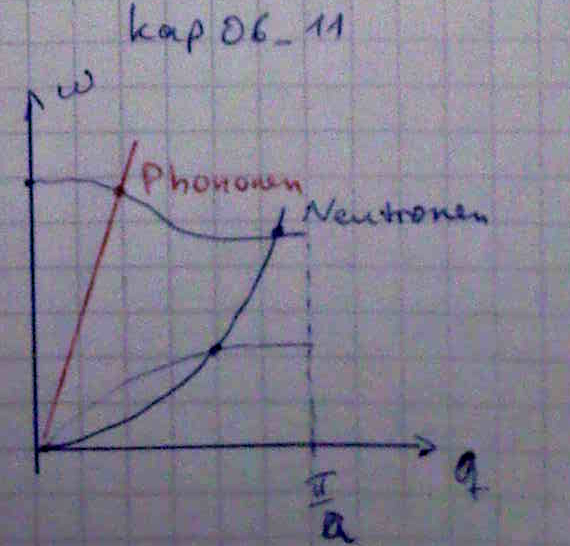
\includegraphics[width=0.75\textwidth]{kap06_11.png}

\section{Zustandsdichte der Phononen}

Theorie eines 3D-Kristalls vorgeschlagen von Born-Karman, 1912 (klassische Theorie)

\(\vec u (x,y,z) = \vec u (x+L_x,y+L_y,z+L_z)\); periodische Randbedingung

Wellen (Moden): \(\vec u = \vec u_0 exp[-i(\omega t-q_xx-q_yy-q_zz)]\)

Periodizität der Atomaren Auslenkung bei \(q_\alpha = m_\alpha\frac{2\pi}{L_\alpha}\); \(\alpha=x,y,z\) und \(m_\alpha\) ganzzahlige Quantenzahl.

\[ e^{iq_\alpha L_\alpha}=1\]

bei einem Kristall mit \(N_\alpha\) Elementarzellen (E.Z.) in \(\alpha\)-Richtung haben wir insgesamt \(N_x,N_y,N_z=N\) E.Z. 3N Lösungen der Bewegungsgleichung; mit p Atome pro E.Z. gibt es 3pN Lösungen der Bewegungsgleichung.

Alle erlaubten wellenvektoren liegen in 1.Brillouin-Zone (1.B.Z.)

'Dichte' \(D(q)\equiv\rho_q\) im reziproken Raum: 

\[\rho_q=\frac{N}{(2\pi)^3/V_z}=\frac{NV_z}{(2\pi)^3}=\frac{V}{(2\pi)^3}\]

\(V_z\)-Das Volumen der E.Z. des realen Gitters.

Zustandsdichte als Funktion der Frequenz \(D(\omega)\): Anzahl von Zuständen pro Einheitsintervall der Frequenz \(\omega\)

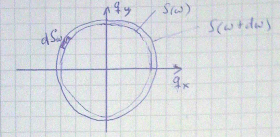
\includegraphics[width=0.75\textwidth]{kap06_12.png}

\[ D(\omega)\cdot d\omega = \rho_q\int^{\omega+d\omega}_\omega d^3q = \rho_q\int^{\omega+d\omega}_\omega dS_\omega\cdot dq_\bot\]

Gruppengeschwindigkeit: \(v_g=\left|\frac{d\omega}{d\vec q}\right| = \left|\underbrace{grad_q\omega}_{\equiv \nabla_q \omega} \right|=\frac{d\omega}{dq_\bot}\)

\[ D(\omega)\cdot d\omega = \frac{V}{(2\pi)^3}\int_{\text{Schalde}\omega=const} \frac{dS_\omega}{v_g}\cdot d\omega\]

Für isotrope Kristalle:

\[ D(\omega)\cdot d\omega = \frac{V}{(2\pi)^3} d\omega \frac{4\pi q^2}{v_g} =\frac{V}{(2\pi)^2} \frac{q^2}{v_g}  d\omega \]

Die Zustandsdichte ist um so größer, je flacher die \(\omega(\vec q)\) verläuft. Kritische Punkte \(\rightarrow\) \underline{van-Hove-Singularitäten} (\(v_g\rightarrow 0\)). Häufigstes vorkommen von Zuständen.

3D \( D(\omega) = \frac{V}{(2\pi)^2} \frac{q^2}{v_g} \); 2D:\( D(\omega) = \frac{A}{(2\pi)^2} \frac{2\pi q^2}{v_g}=\frac{Aq}{2\pi v_g}\) 1D: \( D_1(\omega) = \frac{L}{2\pi}  \frac{2}{v_g}=\frac{L}{\pi v_g} \)

\section{Spezifische Wärme}

\( c=c_{Ges} \frac{N_A}{N}\); \(N_A = 6,022\cdot 10^{23}\); N Elementarzellen E.Z.

\(\left. c\right|_{P=const.}c_p>\left. c\right|_{V=const.}=c_V\); Unterschied zwischen \(c_p\) und \(c_V\) ist in der Realität minimal.

Klassische Theorie: \(c_V = \frac{\partial}{\partial T} U(T)\); \(U\)-innere Energie. Therm. Mittelwert der Energiewerte: \(U\equiv \langle E \rangle = \sum_i p_i\cdot E_i\); \(p_i\)-Wahrscheinlichkeit. Klassisch:

\[ \langle E\rangle = \frac{\int E e^{-\frac{E}{k_B T}}d\Gamma}{\int e^{-\frac{E}{k_B T}}d\Gamma}\]

\(d\Gamma=dx\cdot dy\cdot dz\)-Phasenraum

harmonischer Oszillator: \(\langle E_{Oszi} \rangle = k_B T\)
3pN Gitterschwingungen: \(c_V = 3pNk_B\) Dulong-Petit-Gesetz (1819)

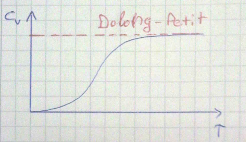
\includegraphics[width=0.75\textwidth]{kap06_13.png}

\(c_V=3R=3\cdot 8,3\frac{J}{mol\cdot K} = 24,9\frac{J}{mol\cdot K} = const.\); \(R\)-univers.Gaskonstante

Quantentheorie: Erste Erklärungsversuch von Einstein (1906) und zweiter und besserer Versuch von Debye (1912). 

Zustand n mit \(E_n=(n+\frac{1}{2})\hbar \omega\); Boltzmann-Verteilung:

\[ p_k=\frac{e^{-\frac{E_n}{k_B T}}}{\sum^\infty_{n=0} e^{-\frac{E_n}{k_B T}}} = e^{-\frac{n \hbar \omega}{k_BT}}\left[1- e^{-\frac{\hbar \omega}{k_BT}}\right]\]


Nenner \(=e^{-\frac{\hbar \omega}{2k_BT}}\sum^\infty_{n=0} \left[e^{-\frac{\hbar \omega}{2k_BT}}\right]^n= e^{-\frac{\hbar \omega}{2k_BT}}\sum^\infty_{n=0} \left[1- e^{-\frac{\hbar \omega}{k_BT}}\right]^{-1}\);mit  \(\sum^\infty_0 x^n = \frac{1-x^{n+1}}{1-x}\approx \frac{1}{1-x}\); \(n\rightarrow \infty,x\rightarrow 0\)


\[ U \equiv \langle E_n \rangle = \sum^\infty_{n=0} p_n\cdot E_n = \left[1- e^{-\frac{\hbar \omega}{k_BT}}\right]\hbar \omega \sum^\infty_{n=0}(n+\frac{1}{2})\left[\underbrace{1- e^{-\frac{\hbar \omega}{k_BT}}}_{x}\right]^n\]

\(\sum_n x^nn=x\frac{d}{dx}\sum_n x^n = \frac{x}{(1-x)^2}\)

\[ \langle E_n \rangle = \hbar \omega \left[ \frac{1}{e^{-\frac{\hbar \omega}{k_BT}}-1}+\frac{1}{2}\right]\]

mit \(E_n=\hbar\omega(n+\frac{1}{2})\)

\(\langle n \rangle \frac{1}{e^{-\frac{\hbar \omega}{k_BT}}-1}\); Bose-Einstein Faktor; \(E(\omega,T) = \hbar \omega[\langle n \rangle + \frac{1}{2}]\)


\section{Debye-Näherung}

Debye-Näherung kann man für isotrope Festkörper anwenden mit \(p=1\Rightarrow \omega = v_g\); \(v=v_g\). Betrachte nur akustische Phononen.

\[  D(\omega)\cdot d\omega = \frac{V}{(2\pi)^2} \frac{\omega^2}{v^3}  d\omega \]

Zustandsdichte pro Phononenzweig (Ast)

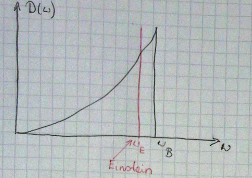
\includegraphics[width=0.75\textwidth]{kap06_14.png}

\(N=\int^{\omega_D}_0\frac{V}{(2\pi)^2} \frac{\omega^2}{v^3}  d\omega = \frac{V\omega^3_D}{6\pi^2 v^3}\); \(\omega_D=\frac{v}{a}\quad ^3\sqrt{6\pi^2}\); \(\frac{V}{N}\approx a^3\)-Gitterkonstante

\(\omega \propto vg\)

Abscheidefrequenz \(\omega_D \Rightarrow\) Debye-Frequenz.
\[\boxed{\omega_D=\frac{v}{a}\quad ^3\sqrt{6\pi^2}}\]

\(D(\omega)= \frac{v\omega^2}{2\pi^2}\left(\frac{1}{v_L^3}+\frac{2}{v^3_T} \right)=\frac{3}{2\pi^2}\frac{\omega^2v}{v_D^3} \); \(\frac{3}{v_D^3}\equiv\frac{1}{v_L^3}+\frac{2}{v_T^3}\); typisch \(v_L\approx \frac{3}{2}v_T\)

Schwingungsenergie des Kristalls: \(v(T) = \int_0^\infty D(\omega) E(\omega,T) d\omega\)

Spezifische Wärme: \(c_V = \frac{\partial v(T)}{\partial T}\); 

\[v=\frac{v}{2\pi^2}\underbrace{\frac{1}{v^3}}_{\frac{3N}{v}\frac{6\pi^2}{\omega_D^3}}\int_0^\infty \omega^2 E(\omega,T) d\omega=\frac{9N}{\omega_D^3}\int_0^\infty\frac{\hbar \omega^3 d\omega}{e^{\frac{\hbar \omega}{k_B T}}-1}\]

Debye-Temperatur: \(\theta_D = \frac{\hbar \omega_D}{k_B}\) mit \(y= \frac{\hbar \omega}{k_BT}\), Debye-Formel:

\[ c_V = 9Nk_B\left(\frac{T}{\theta_D}\right)^3 \int_0^{\theta_D/T}\frac{y^4e^ydy}{(e^y-1)^2}\]


Debye-Temperaturen:

\begin{tabular}{c|ccccccc}
 &\(C_{\text{Diamant}}\)&Be&Si&Al&Cu&Ar&He\\
\(\theta_D,K\)&2230&1000&640&430&340&92&25
\end{tabular}

a) \(T<<\theta_D\) tiefen Temperaturen \(\rightarrow\) Einstein-Theorie
b) \(T>>\theta_D\) hohen Temperatruren  \(\rightarrow\) klassische Thermodynamik

a): \(y\rightarrow \infty\), \(\int_0^\infty \frac{y^4e^ydy}{(e^y-1)^2} = \frac{4\pi^4}{15}\); \(c_v = \frac{12\pi^4}{5}Nk_B\left(\frac{T}{\theta_D}\right)^3 \approx T^3\); \(T^3\)-Gesetz

b): \(y\rightarrow 0\) , \(\int_0^{\theta_D/T}...dy \approx = \int_0^{\theta_D/T}\frac{y^4\cdot 1}{(1+y-1)}dy= \int_0^{\theta_D/T}y^2dy=\frac{1}{3}\left(\frac{T}{\theta_D}\right)^3\), \(c_V=3Nk_B\), Dulong-Petit Gesetz.

\section{Anharmonische Effekte}

Klassisch gesehen ein Anharmonischer Effekt ist eine Abweichung von harmonischen Potential. 

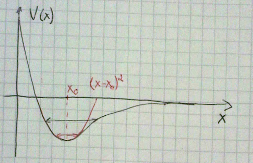
\includegraphics[width=0.75\textwidth]{kap06_15.png}

Auslenkungen sind nicht mehr klein! dann bekommt man die anharmonische Effekte. 

Quantenmechanisch die Anharmonischen Effekte kann man als Wechselwirkung zwischen Phononen beschreiben (Phononenstoßprozesse)

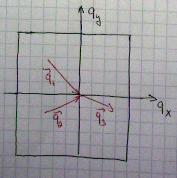
\includegraphics[width=0.75\textwidth]{kap06_16.png}

Normale Prozesse: \(\vec q_1+\vec q_2=\vec q_3\)

Umklapp-Prozesse: \(\vec q_1+\vec q_2=\vec q_3+\vec B\)

\subsection{Therminsche Ausdehnung}
klassisch: \(U(x)\approx cx^2-\overbrace{gx^3-fx^4}^{\text{anharmonische Terme}}+...\);Auslenkung: \(\langle x\rangle = \frac{\int_0^\infty dx x e^{\frac{-U(x)}{k_BT}}}{\int_0^\infty dx e^{\frac{-U(x)}{k_BT}}}\) aus der Thermodynamik ergibt sich:

\[\rightarrow \langle x \rangle \approx \frac{3g}{4c^2}k_B T\]

Wärmeausdehnungskoeffizient:  \(\alpha\equiv \frac{1}{l} \left( \frac{\partial l}{\partial T}\right)_p=\frac{1}{3} \frac{1}{v}\left( \frac{\partial v}{\partial T}\right)_p\); \(l\propto \langle x \rangle\);
  \(\left( \frac{\partial V}{\partial T}\right)_p=-\left( \frac{\partial V}{\partial p}\right)_T\cdot \left( \frac{\partial p}{\partial T}\right)_v\); \(\frac{1}{B}=-\frac{1}{V}\left( \frac{\partial V}{\partial p}\right)_T\)


\(\left( \frac{\partial V}{\partial T}\right)_p = \frac{V}{B}\left( \frac{\partial p}{\partial T}\right)_V\); 

\[\boxed{\alpha = \frac{1}{3B}\left( \frac{\partial p}{\partial T}\right)_V }\]


\( p = - \left( \frac{\partial F}{\partial T}\right)_T\); \(F\)-freie Energie;

 \[ p = -\frac{\partial}{\partial V}(E_0+E_z) -\sum_q\frac{\partial(\hbar \omega_g)}{\partial V}\langle n_g(T)\rangle\] 


\(E_0\)-Energie des Grundzustands; \(E_z\)-Nullpunkt-Schwingungn \(\langle n_g(T)\rangle\)-Mittlere Zahl von Phononen

für harmonischen Kristall: \(c_P=c_V\)

 
\[\alpha = \frac{1}{3B}\sum_q\left[-\frac{V}{\omega_g}\frac{\partial \omega_g}{\partial V}  \right]\underbrace{\frac{1}{V}\hbar \omega_g\frac{\partial}{\partial T}\langle n_g(T)\rangle}_{c_v(q)}\]
\[ = \frac{\partial(ln\omega_g)}{\partial V} \equiv \gamma_q\]

\(\gamma_q\)-Grüneisenzahl
Grüneisenparameter \(\gamma_q\equiv \frac{1}{c_V}\sum_q\gamma_qc_V(q)\approx const. \approx 1\div 3\)

\[\boxed{\alpha = \frac{\gamma c_V}{3B}\approx 10^{-5}K^{-1}}\]

\(\alpha\approx T^3\) für \(T<<\theta_D\); \(\alpha\approx const\) für \(T>>\theta_D\)

\subsection{Wärmeleitfähigkeit}

\[ \kappa = \kappa^{ph}+\kappa^{el}\]

Wärmestromdichte \(\vec J_T = -\kappa\nabla T\), nach den kinetischer Gastheorie \(\kappa = \frac{1}{3}vlc_v = \frac{1}{3}v^2\tau c_v\); \(l\)-Länge; \(\tau\)-mittlere Zeit zur Phononenstöße



\end{document}
